\documentclass[tikz,border=0pt]{standalone}
\usepackage[T1]{fontenc}
\usepackage{lmodern}
\usetikzlibrary{arrows.meta,backgrounds,fit,positioning}
\definecolor{ink}{HTML}{27313A}
\definecolor{pale}{HTML}{F3F5F6}
\tikzset{relation/.style={draw=ink,line width=.6pt},
edge label/.style={font=\sffamily\fontsize{8.5}{10}\selectfont,fill=white,inner sep=1pt},
heading/.style={font=\sffamily\bfseries\fontsize{10}{12}\selectfont,text=ink}}
\begin{document}
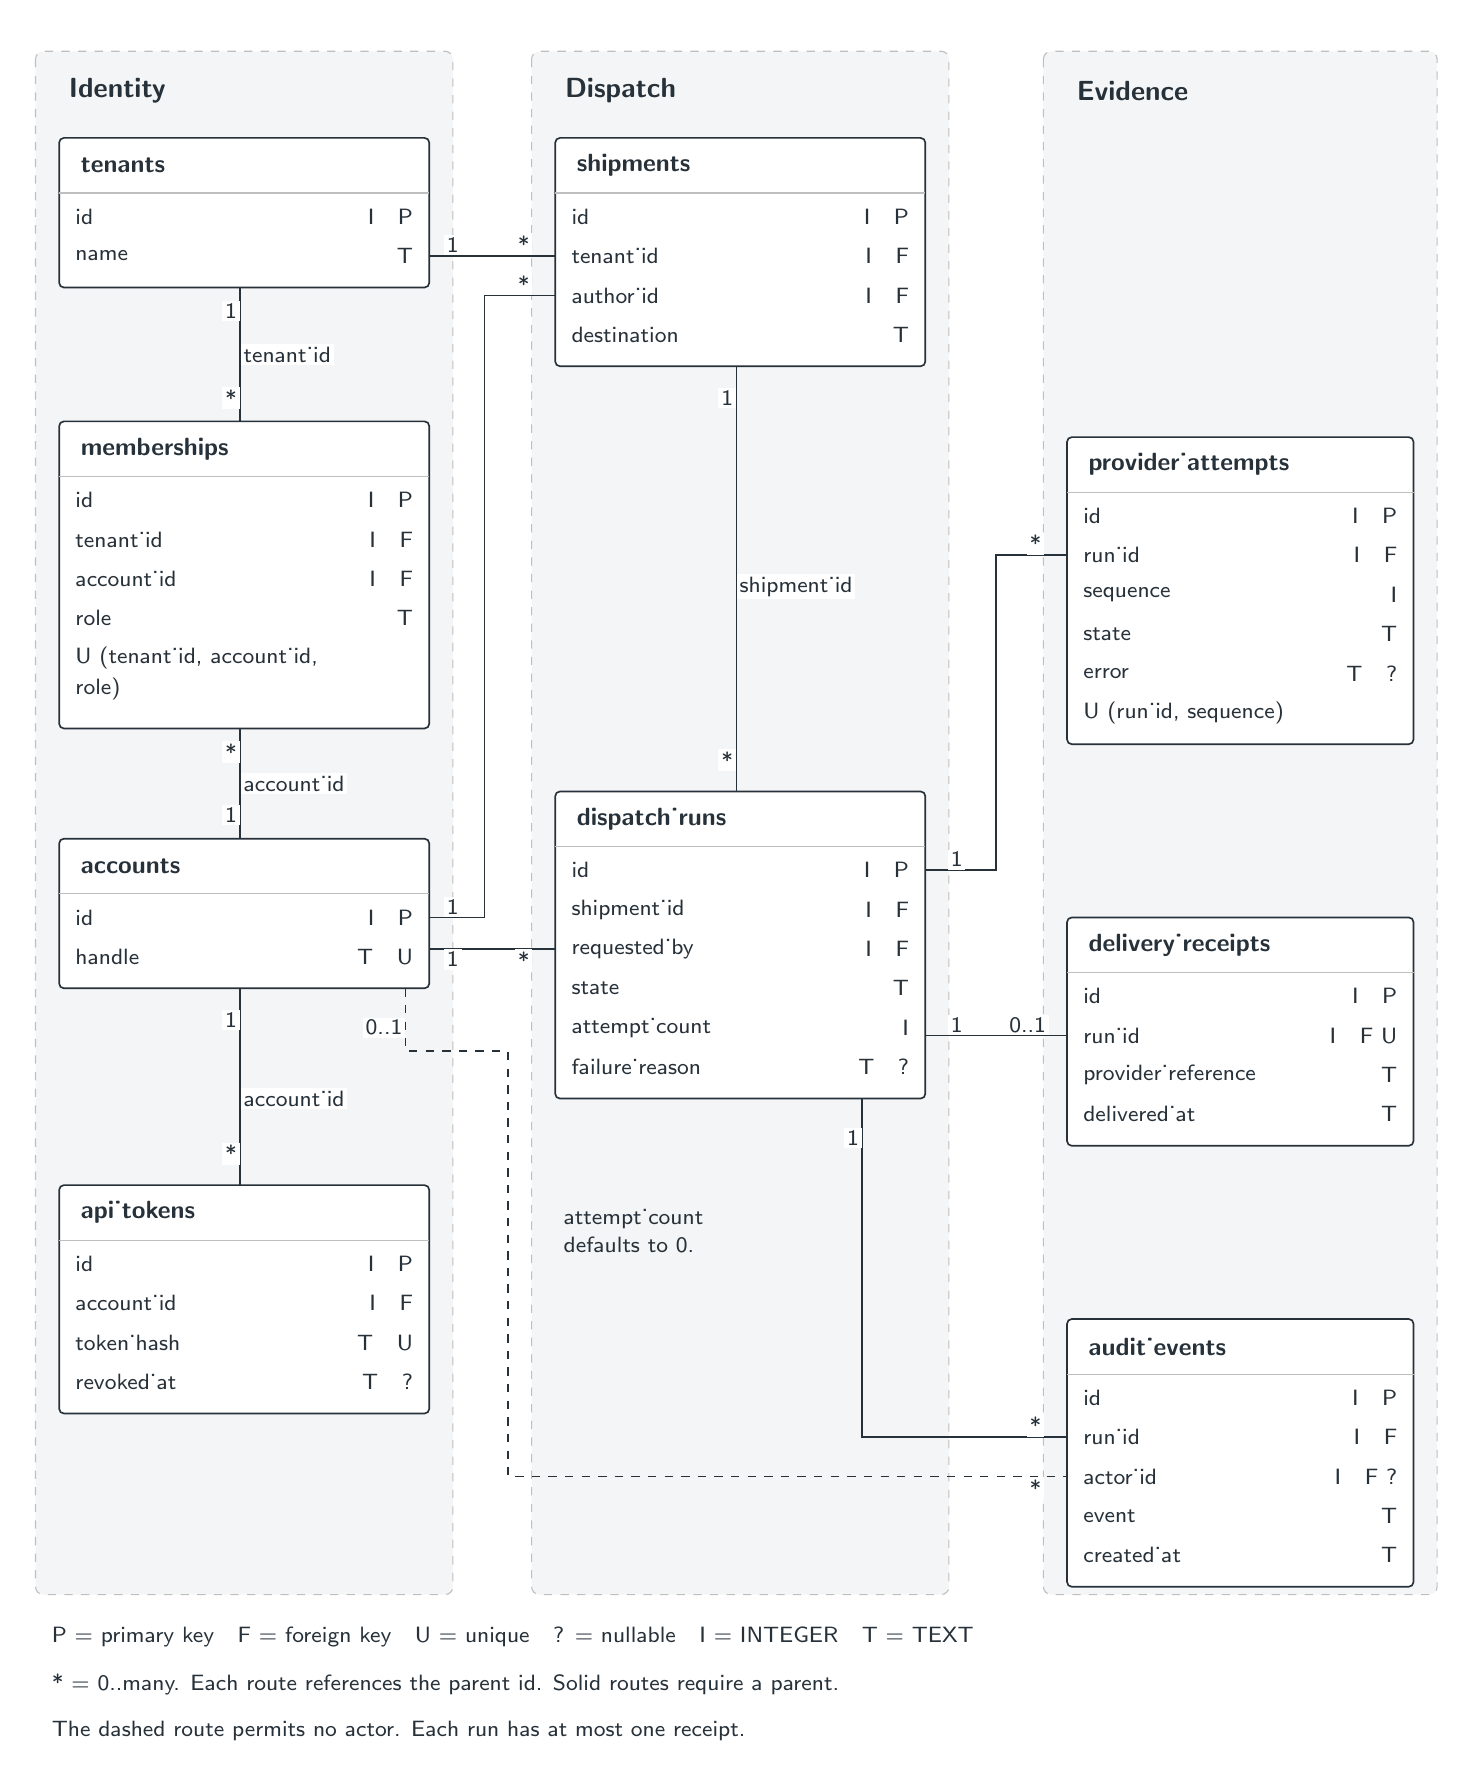
\begin{tikzpicture}[x=1mm,y=-1mm,font=\sffamily\fontsize{8.5}{10}\selectfont,text=ink]
\path[use as bounding box] (0,0) rectangle (180,219);
\draw[draw=black!25,dashed,rounded corners=1mm,fill=pale] (1,3) rectangle (54,199);
\node[heading,anchor=west] at (4,8) {Identity};
\draw[draw=black!25,dashed,rounded corners=1mm,fill=pale] (64,3) rectangle (117,199);
\node[heading,anchor=west] at (67,8) {Dispatch};
\draw[draw=black!25,dashed,rounded corners=1mm,fill=pale] (129,3) rectangle (179,199);
\node[heading,anchor=west] at (132,8) {Evidence};
\draw[fill=white,draw=ink,line width=.6pt,rounded corners=.6mm] (4,14) rectangle (51,33);
\node[anchor=west,font=\sffamily\bfseries\fontsize{9}{11}\selectfont] at (5.5,17.5) {\detokenize{tenants}};
\draw[draw=black!25] (4,21) -- (51,21);
\node[anchor=west,inner sep=0] at (6,24) {\detokenize{id}};
\node[anchor=east,inner sep=0] at (49,24) {I\quad P};
\node[anchor=west,inner sep=0] at (6,29) {\detokenize{name}};
\node[anchor=east,inner sep=0] at (49,29) {T\quad };
\draw[fill=white,draw=ink,line width=.6pt,rounded corners=.6mm] (4,50) rectangle (51,89);
\node[anchor=west,font=\sffamily\bfseries\fontsize{9}{11}\selectfont] at (5.5,53.5) {\detokenize{memberships}};
\draw[draw=black!25] (4,57) -- (51,57);
\node[anchor=west,inner sep=0] at (6,60) {\detokenize{id}};
\node[anchor=east,inner sep=0] at (49,60) {I\quad P};
\node[anchor=west,inner sep=0] at (6,65) {\detokenize{tenant_id}};
\node[anchor=east,inner sep=0] at (49,65) {I\quad F};
\node[anchor=west,inner sep=0] at (6,70) {\detokenize{account_id}};
\node[anchor=east,inner sep=0] at (49,70) {I\quad F};
\node[anchor=west,inner sep=0] at (6,75) {\detokenize{role}};
\node[anchor=east,inner sep=0] at (49,75) {T\quad };
\node[anchor=west,inner sep=0] at (6,80) {\detokenize{U (tenant_id, account_id,}};
\node[anchor=west,inner sep=0] at (6,84) {\detokenize{role)}};
\draw[fill=white,draw=ink,line width=.6pt,rounded corners=.6mm] (4,103) rectangle (51,122);
\node[anchor=west,font=\sffamily\bfseries\fontsize{9}{11}\selectfont] at (5.5,106.5) {\detokenize{accounts}};
\draw[draw=black!25] (4,110) -- (51,110);
\node[anchor=west,inner sep=0] at (6,113) {\detokenize{id}};
\node[anchor=east,inner sep=0] at (49,113) {I\quad P};
\node[anchor=west,inner sep=0] at (6,118) {\detokenize{handle}};
\node[anchor=east,inner sep=0] at (49,118) {T\quad U};
\draw[fill=white,draw=ink,line width=.6pt,rounded corners=.6mm] (4,147) rectangle (51,176);
\node[anchor=west,font=\sffamily\bfseries\fontsize{9}{11}\selectfont] at (5.5,150.5) {\detokenize{api_tokens}};
\draw[draw=black!25] (4,154) -- (51,154);
\node[anchor=west,inner sep=0] at (6,157) {\detokenize{id}};
\node[anchor=east,inner sep=0] at (49,157) {I\quad P};
\node[anchor=west,inner sep=0] at (6,162) {\detokenize{account_id}};
\node[anchor=east,inner sep=0] at (49,162) {I\quad F};
\node[anchor=west,inner sep=0] at (6,167) {\detokenize{token_hash}};
\node[anchor=east,inner sep=0] at (49,167) {T\quad U};
\node[anchor=west,inner sep=0] at (6,172) {\detokenize{revoked_at}};
\node[anchor=east,inner sep=0] at (49,172) {T\quad ?};
\draw[fill=white,draw=ink,line width=.6pt,rounded corners=.6mm] (67,14) rectangle (114,43);
\node[anchor=west,font=\sffamily\bfseries\fontsize{9}{11}\selectfont] at (68.5,17.5) {\detokenize{shipments}};
\draw[draw=black!25] (67,21) -- (114,21);
\node[anchor=west,inner sep=0] at (69,24) {\detokenize{id}};
\node[anchor=east,inner sep=0] at (112,24) {I\quad P};
\node[anchor=west,inner sep=0] at (69,29) {\detokenize{tenant_id}};
\node[anchor=east,inner sep=0] at (112,29) {I\quad F};
\node[anchor=west,inner sep=0] at (69,34) {\detokenize{author_id}};
\node[anchor=east,inner sep=0] at (112,34) {I\quad F};
\node[anchor=west,inner sep=0] at (69,39) {\detokenize{destination}};
\node[anchor=east,inner sep=0] at (112,39) {T\quad };
\draw[fill=white,draw=ink,line width=.6pt,rounded corners=.6mm] (67,97) rectangle (114,136);
\node[anchor=west,font=\sffamily\bfseries\fontsize{9}{11}\selectfont] at (68.5,100.5) {\detokenize{dispatch_runs}};
\draw[draw=black!25] (67,104) -- (114,104);
\node[anchor=west,inner sep=0] at (69,107) {\detokenize{id}};
\node[anchor=east,inner sep=0] at (112,107) {I\quad P};
\node[anchor=west,inner sep=0] at (69,112) {\detokenize{shipment_id}};
\node[anchor=east,inner sep=0] at (112,112) {I\quad F};
\node[anchor=west,inner sep=0] at (69,117) {\detokenize{requested_by}};
\node[anchor=east,inner sep=0] at (112,117) {I\quad F};
\node[anchor=west,inner sep=0] at (69,122) {\detokenize{state}};
\node[anchor=east,inner sep=0] at (112,122) {T\quad };
\node[anchor=west,inner sep=0] at (69,127) {\detokenize{attempt_count}};
\node[anchor=east,inner sep=0] at (112,127) {I\quad };
\node[anchor=west,inner sep=0] at (69,132) {\detokenize{failure_reason}};
\node[anchor=east,inner sep=0] at (112,132) {T\quad ?};
\draw[fill=white,draw=ink,line width=.6pt,rounded corners=.6mm] (132,52) rectangle (176,91);
\node[anchor=west,font=\sffamily\bfseries\fontsize{9}{11}\selectfont] at (133.5,55.5) {\detokenize{provider_attempts}};
\draw[draw=black!25] (132,59) -- (176,59);
\node[anchor=west,inner sep=0] at (134,62) {\detokenize{id}};
\node[anchor=east,inner sep=0] at (174,62) {I\quad P};
\node[anchor=west,inner sep=0] at (134,67) {\detokenize{run_id}};
\node[anchor=east,inner sep=0] at (174,67) {I\quad F};
\node[anchor=west,inner sep=0] at (134,72) {\detokenize{sequence}};
\node[anchor=east,inner sep=0] at (174,72) {I\quad };
\node[anchor=west,inner sep=0] at (134,77) {\detokenize{state}};
\node[anchor=east,inner sep=0] at (174,77) {T\quad };
\node[anchor=west,inner sep=0] at (134,82) {\detokenize{error}};
\node[anchor=east,inner sep=0] at (174,82) {T\quad ?};
\node[anchor=west,inner sep=0] at (134,87) {\detokenize{U (run_id, sequence)}};
\draw[fill=white,draw=ink,line width=.6pt,rounded corners=.6mm] (132,113) rectangle (176,142);
\node[anchor=west,font=\sffamily\bfseries\fontsize{9}{11}\selectfont] at (133.5,116.5) {\detokenize{delivery_receipts}};
\draw[draw=black!25] (132,120) -- (176,120);
\node[anchor=west,inner sep=0] at (134,123) {\detokenize{id}};
\node[anchor=east,inner sep=0] at (174,123) {I\quad P};
\node[anchor=west,inner sep=0] at (134,128) {\detokenize{run_id}};
\node[anchor=east,inner sep=0] at (174,128) {I\quad F U};
\node[anchor=west,inner sep=0] at (134,133) {\detokenize{provider_reference}};
\node[anchor=east,inner sep=0] at (174,133) {T\quad };
\node[anchor=west,inner sep=0] at (134,138) {\detokenize{delivered_at}};
\node[anchor=east,inner sep=0] at (174,138) {T\quad };
\draw[fill=white,draw=ink,line width=.6pt,rounded corners=.6mm] (132,164) rectangle (176,198);
\node[anchor=west,font=\sffamily\bfseries\fontsize{9}{11}\selectfont] at (133.5,167.5) {\detokenize{audit_events}};
\draw[draw=black!25] (132,171) -- (176,171);
\node[anchor=west,inner sep=0] at (134,174) {\detokenize{id}};
\node[anchor=east,inner sep=0] at (174,174) {I\quad P};
\node[anchor=west,inner sep=0] at (134,179) {\detokenize{run_id}};
\node[anchor=east,inner sep=0] at (174,179) {I\quad F};
\node[anchor=west,inner sep=0] at (134,184) {\detokenize{actor_id}};
\node[anchor=east,inner sep=0] at (174,184) {I\quad F ?};
\node[anchor=west,inner sep=0] at (134,189) {\detokenize{event}};
\node[anchor=east,inner sep=0] at (174,189) {T\quad };
\node[anchor=west,inner sep=0] at (134,194) {\detokenize{created_at}};
\node[anchor=east,inner sep=0] at (174,194) {T\quad };

% Each route joins a parent table to a child table.
% Horizontal child ports align with their foreign key rows.
\draw[relation] (51,29) -- (67,29);
\node[edge label,above] at (54,29) {1};
\node[edge label,above] at (63,29) {*};
\draw[relation] (27,33) -- (27,50);
\node[edge label,left] at (27,36) {1};
\node[edge label,left] at (27,47) {*};
\node[edge label,right] at (27,41.5) {\detokenize{tenant_id}};
\draw[relation] (27,89) -- (27,103);
\node[edge label,left] at (27,92) {*};
\node[edge label,left] at (27,100) {1};
\node[edge label,right] at (27,96) {\detokenize{account_id}};
\draw[relation] (27,122) -- (27,147);
\node[edge label,left] at (27,126) {1};
\node[edge label,left] at (27,143) {*};
\node[edge label,right] at (27,136) {\detokenize{account_id}};
\draw[relation] (51,113) -- (58,113) -- (58,34) -- (67,34);
\node[edge label,above] at (54,113) {1};
\node[edge label,above] at (63,34) {*};
\draw[relation] (51,117) -- (67,117);
\node[edge label,below] at (54,117) {1};
\node[edge label,below] at (63,117) {*};
\draw[relation] (90,43) -- (90,97);
\node[edge label,left] at (90,47) {1};
\node[edge label,left] at (90,93) {*};
\node[edge label,right] at (90,71) {\detokenize{shipment_id}};
\draw[relation] (114,107) -- (123,107) -- (123,67) -- (132,67);
\node[edge label,above] at (118,107) {1};
\node[edge label,above] at (128,67) {*};
\draw[relation] (114,128) -- (132,128);
\node[edge label,above] at (118,128) {1};
\node[edge label,above] at (127,128) {0..1};
\draw[relation] (106,136) -- (106,179) -- (132,179);
\node[edge label,left] at (106,141) {1};
\node[edge label,above] at (128,179) {*};
\draw[relation,dashed] (48,122) -- (48,130) -- (61,130) -- (61,184) -- (132,184);
\node[edge label,left] at (48,127) {0..1};
\node[edge label,below] at (128,184) {*};
\node[anchor=north west,align=left,inner sep=0] at (68,150) {\detokenize{attempt_count}\\defaults to 0.};
\node[anchor=north west,align=left,inner sep=0] at (3,203) {P = primary key\quad F = foreign key\quad U = unique\quad ? = nullable\quad I = INTEGER\quad T = TEXT};
\node[anchor=north west,align=left,inner sep=0] at (3,209) {* = 0..many. Each route references the parent id. Solid routes require a parent.};
\node[anchor=north west,align=left,inner sep=0] at (3,215) {The dashed route permits no actor. Each run has at most one receipt.};
\end{tikzpicture}
\end{document}
